\chapter{Case Squashing}
\label{cha:case_squashing}

\section{Usage}

We added the option:

\begin{verbatim}
--squash-cases                              remove unnecessary case expressions
\end{verbatim}

to our Agda branch which, when enabled, will perform the case squashing optimisation described above.

\section{Logical Representation}

The goal of case squashing is to eliminate case expressions where the scrutinee has already been matched on by an enclosing ancestor case expression. Figure~\ref{fig:case_squash_rule} shows the transformation from a case expression with repeated scrutinisations on the same variable, to the optimised ``case squashed'' version.

\begin{figure}[h]
\centering
\begin{subfigure}{.47\textwidth}
  \centering
  \begin{lstlisting}[style=math]
  case $i : \tau$ of
   $d~(ar-1)~..~0 \to$
     ...
       case $j : \tau$ of
         $d~(ar-1)~..~0 \to r$
  \end{lstlisting}
  where \lstinline[style=math]{lookupVar($i$) = lookupVar($j$)}.
\end{subfigure}
{\large$\to$}
\begin{subfigure}{.47\textwidth}
  \centering
  \begin{lstlisting}[style=math]
  case $i : \tau$ of
   $d~(ar-1)~..~0 \to$
     ...
       $r'$
  \end{lstlisting}
  where $r'$ is $r$ with variables $0, ..., (ar-1)$ replaced with the corresponding bound variables from the ancestor case expression.
\end{subfigure}
\caption{Case squashing rule.}
\label{fig:case_squash_rule}
\end{figure}

For example, given the following simplified treeless expression:

\begin{lstlisting}[style=math]
$\lambda~\textcolor{red}{0} \to$
$\lambda~0 \to$
$\lambda~0 \to$
case $\textcolor{red}{2}$ of
  $da~2~1~0 \to$
    case $0$ of
      $db~1~0 \to$
        case $\textcolor{red}{7}$ of
          $da~2~1~0 \to r$
          ...
      ...
  ...
\end{lstlisting}

we can follow the de Bruijn indices to their matching variable bindings, to see that the first and third case expressions are scrutinising the same variable, the one bound by the outermost $\lambda$ abstraction. Therefore, with only static analysis of the expression tree, we know that the third case expression must follow the $da~2~1~0$ branch, and we can thus safely transform our expression into the following substituted expression:

\begin{lstlisting}[style=math]
$\lambda~0 \to$
$\lambda~0 \to$
$\lambda~0 \to$
case $2$ of {
  $da~\textcolor{red}{2}~\textcolor{blue}{1}~\textcolor{green}{0} \to$
    case $0$ of
      $db~1~0 \to$
        $r[2 := \textcolor{red}{4}, 1 := \textcolor{blue}{3}, 0 := \textcolor{green}{2}]$
      ...
  ...
\end{lstlisting}

We perform this ``case squashing'' by accumulating an environment of all previously scrutinised variables as we traverse the tree structure (appropriately shifting de Bruijn indices in the environment as new variables are bound), and replacing case expressions that match on the same variable as an ancestor case expressions, with the corresponding case branch's body. Any variables in the body that refer to bindings in the removed branch should be replaced with references to the bindings in the matching ancestor case expression branch.

\section{Implementation}

The case squashing implementation is practically very similar to it's logical representation described above. While recursing through the treeless structure we accumulate an environment containing the relevant attributes of the case expressions in scope. As new variables are bound recursing down the structure, the indices stored in this environment are incremented accordingly.

For more details about how variable indices are replaced in the resulting term, refer to section~\ref{sub:lambda_calc_subst}.

For a complete listing of our implementation of the case squashing optimisation, refer to Appendix~\ref{app:case_squash}.

\section{Application}

\input{Figures/Agda/latex/Example1}

Take for example the simple usage of record projections in Figure~\ref{code:example1_agda}. When we compile this module once without \texttt{-{}-inline-proj} on, and once again with \texttt{-{}-inline-proj} enabled, a unified diff of the two generated Haskell files gives us what is shown in Figure~\ref{fig:Example1_inline}.

\begin{figure}[h!]
    \centering
    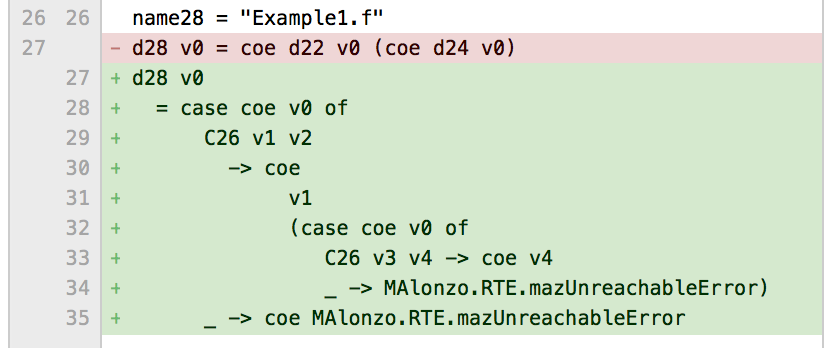
\includegraphics[width=0.5\textwidth]{Figures/Example1_inline}
    \caption{Unified difference of the \AgdaModule{Example1}~module compiled without and then with \texttt{-{}-inline-proj}.}
    \label{fig:Example1_inline}
\end{figure}

The compiled projection function \AgdaField{Pair.snd}, that is \lstinline{d18} in the Haskell code, is replaced with a Haskell expression that cases on the pair (\AgdaFunction{p} in Agda, \lstinline{d22} in Haskell) and returns the second field.

\begin{figure}[h!]
    \centering
    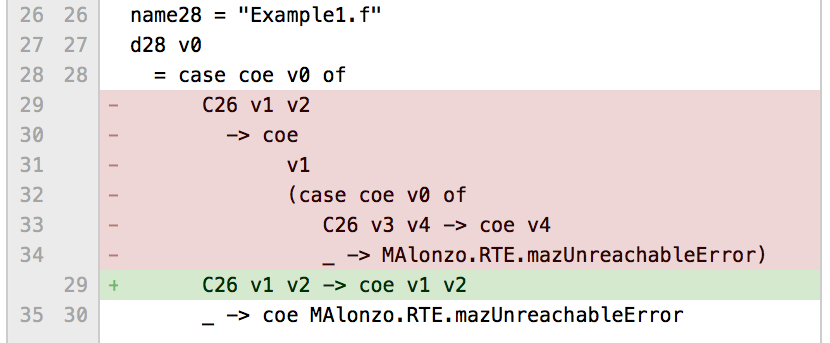
\includegraphics[width=0.5\textwidth]{Figures/Example1_squash}
    \caption{Unified difference of the \AgdaModule{Example1}~module compiled  with \texttt{-{}-inline-proj} and then also with \texttt{-{}-squash-cases}.}
    \label{fig:Example1_squash}
\end{figure}

We then compile the same file with both \texttt{-{}-inline-proj} and \texttt{-{}-squash-cases}, and the difference between only inlining and both inlining and squashing can be seen in Figure~\ref{fig:Example1_squash}.

\begin{figure}[h!]
    \centering
    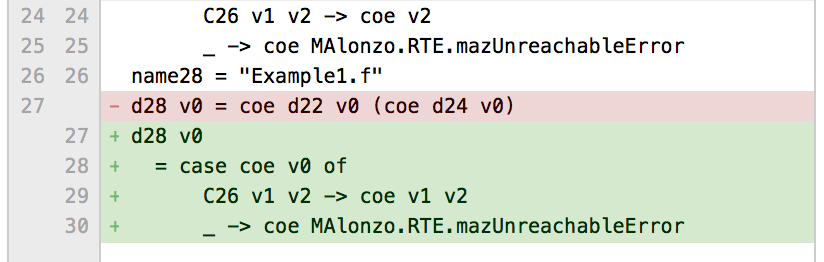
\includegraphics[width=0.5\textwidth]{Figures/Example1_inline_squash}
    \caption{Unified difference of the \AgdaModule{Example1}~module compiled without either optimisation, then with both \texttt{-{}-inline-proj} and \texttt{-{}-squash-cases}.}
    \label{fig:Example1_inline_squash}
\end{figure}

Figure~\ref{fig:Example1_inline_squash} shows the overall unified diff from neither optimisation to both.
